\documentclass[11pt]{article}
\usepackage{amsmath,amssymb,amsthm}
\usepackage[letterpaper,margin=1in]{geometry}
\usepackage{microtype}
\usepackage{graphicx}
\usepackage[hidelinks]{hyperref}
\newtheorem{theorem}{Theorem}
\newtheorem{lemma}[theorem]{Lemma}
\newtheorem{corollary}[theorem]{Corollary}
\newcommand{\F}{\mathbb F}
\newcommand{\E}{\mathbb E}
\newcommand{\Prob}{\mathbb P}
\newcommand{\ind}{\mathbf 1}
\newcommand{\OPT}{\operatorname{OPT}}
\title{Covering versus hitting in diversity embeddings:\\an affine obstruction and matching bounds}
\author{Jeff Kline}
\date{Version 0.1.0 --- September 13, 2026\\[3pt]\small\href{https://doi.org/10.5281/zenodo.22731697}{doi:10.5281/zenodo.22731697}}
\hypersetup{pdftitle={Covering versus hitting in diversity embeddings: an affine obstruction and matching bounds},pdfauthor={Jeff Kline}}
\begin{document}
\maketitle
\begin{abstract}
For every prime power $q$, we construct a unit-length hypergraph on $q^2+1$
vertices whose minimum $\ell_1$ diversity distortion lies between
$q^2/(2q-1)$ and $q$, using $q^2$ supplies and $O(q^3\log q)$ encoding bits.
The square-root lower bound and its finite constant already follow from
prior set-function work via exponentially many supplies; priority of the
compact realization remains unresolved. Its encoding size contradicts
Conjecture 1.7 of Jozefiak and Shepherd in arXiv:2303.04199v1, and the
specified connector LP has the same integrality-gap lower bound.
The proof compares covering cost with hitting probabilities through
incidence moments. Conversely, established universal set-cover
approximations give distortion at most $4\sqrt n$ for unit-cost
pairwise-intersecting supply hypergraphs, even without a common root.
The square-root exponent is tight in this class, including families with
empty global intersection. Positive costs in this class give an upper
bound $2\sqrt{nH_n}$, where $H_n$ is the $n$th harmonic number.
These upper bounds do not settle arbitrary hypergraphs. A constant-factor
coverage approximation for a known greedy-bad family separates that
algorithm's logarithmic loss from a diversity-embedding obstruction.
\end{abstract}

\section{The covering--hitting principle}
A diversity, introduced by Bryant and Tupper~\cite{BT12}, generalizes a
metric by assigning a nonnegative value to each finite set of points,
subject to a generalized triangle inequality. An $\ell_1$ diversity measures
this value by summing coordinate ranges. Here the value of a terminal set is
the minimum cost of a connected supply collection spanning it. A cut indicator asks only whether terminals occur on both sides
of a cut. When cheap supplies and expensive demands have comparable
crossing probabilities for every cut, no nonnegative cut mixture can
approximate both costs well. This is the mechanism behind the example
below; its affine incidence structure supplies a small explicit witness.
Covering multiplicity alone is insufficient: the probability comparison
must hold uniformly over cuts under the same supply and demand measures.

An existential square-root lower bound for diversities already follows
from the set-function separation of Badanidiyuru et al.~\cite{SVF} by a
rooted construction with exponentially many supplies, as explained in
Section~\ref{sec:related}. The distinction here is the explicit polynomial-size
supply representation, its encoding-size consequence, and the specified LP gap.
The same prior proof also yields the finite constant $q^2/(2q-1)$.
Priority of the precise compact contribution remains unresolved.

This investigation grew out of range-cost multi-marginal earth moving.
Kline~\cite{K19} established geometric properties of its value, including
convex-hull monotonicity and Minkowski additivity. The subsequent prefix-width
study~\cite{K26} expresses the value as the sum, over cuts between adjacent
bins, of the largest cumulative mass minus the smallest. In cumulative
coordinates this is precisely the coordinate-range $\ell_1$ diversity.
That connection led to the embedding question studied here and to examining
what nonnegative cut sums can detect. The present obstruction uses the
standard cut representation directly; it does not require the later
transport-rigidity theorem. These works provide the geometric starting
point, while the covering--hitting argument supplies the obstruction.

The matching question has a complete answer for a substantial special
class. If supply edges pairwise intersect, every cover is connected.
We transfer established universal set-cover approximations to diversity
embeddings on all terminal sets, obtaining the square-root exponent for
unit costs. These upper bounds do not settle the corresponding question
for arbitrary hypergraphs. In general, the ratio between minimum connected
cost and minimum cover cost can grow without bound, so the transfer does
not give a uniform approximation for arbitrary hypergraphs. Controlling
that ratio or finding a different transfer is a separate obstacle from
removing the weighted logarithm, and the general square-root direction
of Bryant and Tupper~\cite{BT17} remains unresolved here.


\section{Definitions and construction}
For a connected hypergraph $G=(V,E)$ with nonnegative edge lengths $\ell_e$,
its \emph{Steiner diversity} is
\[
 \delta_G(A)=\min_{J\in\mathcal T_A}\sum_{e\in J}\ell_e
 \quad (|A|\ge2),
\]
where $\mathcal T_A$ consists of edge subsets inducing a connected
subhypergraph containing $A$. Connectivity is incidence connectivity;
vertices outside $A$ may be used. Set $\delta_G(A)=0$ for $|A|\le1$.
This is the convention in \cite[Definition 1.6]{JS}.

For a map $f:V\to\mathbb R^d$, the induced $\ell_1$ diversity is the
sum of coordinate ranges,
\[
 \Delta_f(A)=\sum_{i=1}^d
 \left(\max_{v\in A}f_i(v)-\min_{v\in A}f_i(v)\right),
\]
with value zero on the empty set. After rescaling, distortion $D$ means
$\delta_G(A)\le\Delta_f(A)\le D\delta_G(A)$ for every $A\subseteq V$.
There is no bound on $d$ in the result below.

Fix a prime power $q$. Let $X=\F_q^2$ and $V=X\cup\{r\}$, where $r$ is a new
root. For $a,b\in\F_q$, put
\[
 L_{a,b}=\{(x,ax+b):x\in\F_q\},\qquad e_{a,b}=\{r\}\cup L_{a,b}.
\]
Take these $q^2$ rooted nonvertical lines as the supply edges, all of length
one. Vertical lines are not supply edges. For $x\in\F_q$, define
\[
 Q_x=\{(x,y):y\in\F_q\},\qquad A_x=\{r\}\cup Q_x.
\]
These rooted columns will serve as the demand sets. Write $\delta_q$ for
the resulting Steiner diversity. The hypergraph has rank $q+1$ and
$q^2(q+1)$ incidences. Listing vertex identifiers and unit lengths takes
$O(q^3\log q)$ bits.

Every nonempty supply-edge collection is connected through $r$. Therefore,
for $|A|\ge2$, $\delta_q(A)$ is exactly the minimum number of nonvertical
lines covering $A\cap X$. In particular,
\begin{equation}\label{eq:costs}
 \delta_q(e_{a,b})=1,\qquad \delta_q(A_x)=q.
\end{equation}
The second equality holds because each supply line meets a column in one
point, and the $q$ horizontal lines cover the entire plane.

\begin{figure}[p]
\centering
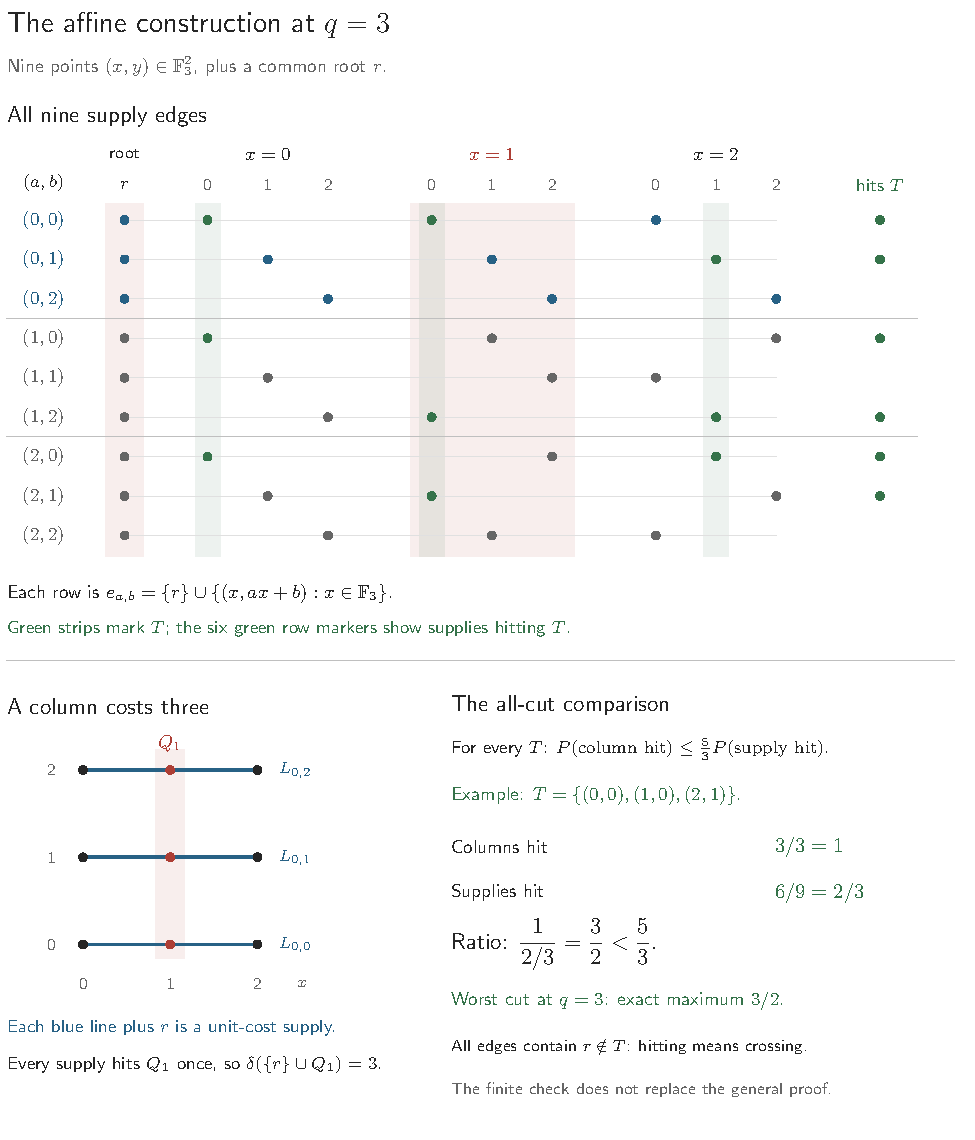
\includegraphics[width=0.97\textwidth]{figures/affine-q3.pdf}
\caption{The construction and hitting comparison at $q=3$.
Every supply contains the root and one point in each column, whereas a
rooted column costs three. The displayed test set hits all three columns
and six of nine supplies, giving ratio $3/2$. Exact enumeration of all
$2^9=512$ test sets (with the empty set handled separately) confirms that
$3/2$ is the maximum for $q=3$, attained by 18 non-collinear triples.
This is a finite check, not a proof for general $q$. The moment bound in
Lemma~\ref{lem:hit} is $C_q=(2q-1)/q$, hence $5/3$ here.
The generator and exact enumeration are included in the repository.}
\label{fig:affine-q3}
\end{figure}


\section{An inequality for every cut}
For $T\subseteq X$, let
\[
 c_T(A)=\ind\{A\cap T\ne\varnothing,\ A\cap(V\setminus T)\ne\varnothing\}.
\]
Every nontrivial cut can be oriented to have its root-free side in $X$.
On a rooted set $\{r\}\cup B$, its value is simply
$\ind\{T\cap B\ne\varnothing\}$.

\begin{lemma}\label{lem:hit}
For every $T\subseteq X$, a uniformly chosen column $Q$ and a uniformly
chosen nonvertical affine line $L$ satisfy
\[
 \Prob(Q\cap T\ne\varnothing)
 \le C_q\Prob(L\cap T\ne\varnothing),\qquad C_q=\frac{2q-1}{q}.
\]
\end{lemma}
\begin{proof}
Suppose $T\ne\varnothing$. Let $t_x=|T\cap Q_x|$, $t=\sum_x t_x$,
and let $h$ be the number of occupied columns. For $Z=|L\cap T|$,
point and ordered-pair incidence counts give
\[
 \E Z=t/q,\qquad
 \E Z^2=t/q+(t^2-\sum_x t_x^2)/q^2.
\]
Distinct points in different columns lie on exactly one supply line;
points in the same column cannot occur together. Cauchy--Schwarz gives
$\Prob(Z>0)\ge(\E Z)^2/\E Z^2$. Since column hitting has probability
$h/q$, its ratio to line hitting is at most
\[
 \frac hq\left(\frac qt+1-\frac{\sum_x t_x^2}{t^2}\right)
 \le\frac hq\left(\frac qt+1-\frac1h\right)
 \le\frac{q+h-1}{q}\le\frac{2q-1}{q}.
\]
Here $\sum_x t_x^2\ge t^2/h$, $t\ge h$, and $h\le q$.
For $T=\varnothing$, both probabilities vanish.
\end{proof}

A finite $\ell_1$ diversity is a nonnegative sum of cut diversities:
\begin{equation}\label{eq:cuts}
 \Delta=\sum_{T\subseteq X}w_Tc_T,\qquad w_T\ge0.
\end{equation}
Indeed, sort the distinct values in each coordinate of an embedding.
Each consecutive gap contributes its length times the cut separating
values above that gap from those below it. These contributions telescope
to the coordinate range on every set. Complement cuts containing $r$,
then sum over coordinates. Conversely, weighted cut indicators give
an $\ell_1$ embedding. This is also the cut representation used in
\cite{BT,JS}.

Multiplying Lemma~\ref{lem:hit} by $w_T$ and summing yields the central
inequality, valid for every nonnegative cut sum:
\begin{equation}\label{eq:average}
 \frac1q\sum_x\Delta(A_x)
 \le \frac{C_q}{q^2}\sum_{a,b}\Delta(e_{a,b}).
\end{equation}

\section{The embedding obstruction}
\begin{theorem}\label{thm:embedding}
The minimum $\ell_1$ diversity distortion of $(V,\delta_q)$ satisfies
\[
 \frac{q^2}{2q-1}\le D_{\min}\le q.
\]
The lower bound already follows from requiring domination on the $q$
sets $A_x$ and the upper bound $\Delta(e_{a,b})\le D$ on the $q^2$
supply edges.
\end{theorem}
\begin{proof}
By \eqref{eq:costs} and \eqref{eq:average}, these restricted constraints imply
\[
 q\le\frac1q\sum_x\Delta(A_x)
   \le\frac{C_q}{q^2}\sum_{a,b}\Delta(e_{a,b})\le C_qD.
\]
For the upper bound, use the unit-weight singleton cuts
$\Delta_0=\sum_{p\in X}c_{\{p\}}$. For $|A|\ge2$, put $s=|A\cap X|$.
Then $\Delta_0(A)=s$. Each supply line covers at most $q$ of these points,
while choosing one line through each point gives a connected cover. Hence
\[
 s/q\le\delta_q(A)\le s,
 \qquad \delta_q(A)\le\Delta_0(A)\le q\delta_q(A).
\]
Both diversities vanish on empty sets and singletons.
\end{proof}

\begin{corollary}
Conjecture 1.7 of \cite{JS}, in its arXiv v1 formulation, is false.
\end{corollary}
\begin{proof}
That conjecture asks for distortion polylogarithmic in the encoding size
of the inducing hypergraph. Here $B_q=O(q^3\log q)$, while the distortion
is at least $q/2$. Along unbounded primes, $q/2$ exceeds
$C\log(2+B_q)^k$ for every fixed $C>0$ and $k\ge0$.
The obstruction concerns existence, independently of running time.
\end{proof}

Since $n=q^2+1$, this family's minimum distortion is $\Theta(\sqrt n)$.
This is a statement about the explicit family; no matching upper bound
for all diversities is claimed.

\section{An explicit connector-LP gap}
Give each supply edge capacity $c_{a,b}=1/q^2$ and each demand edge $A_x$
weight $b_x=1/q$. These capacities are distinct from the unit lengths used
to define $\delta_q$. For a nontrivial cut with root-free side $T$, its ratio is
\[
 \phi(T)=\frac{q^{-2}\sum_{a,b}c_T(e_{a,b})}
                   {q^{-1}\sum_x c_T(A_x)}.
\]
The denominator is positive because nonempty $T$ meets a column.
Lemma~\ref{lem:hit} gives $\phi(T)\ge1/C_q=q/(2q-1)$.

The connector relaxation \cite[Equation (24)]{JS} specializes to
\begin{equation}\label{eq:lp}
\begin{aligned}
 \text{minimize}\quad &q^{-2}\sum_{a,b}d_{a,b}\\
 \text{subject to}\quad &q^{-1}\sum_x y_x\ge1,\\
 &\sum_{e_{a,b}\in J}d_{a,b}\ge y_x
       &&(x\in\F_q,\ J\in\mathcal T_{A_x}),\\
 &d_{a,b}\ge0,\quad y_x\ge0.
\end{aligned}
\end{equation}
For completeness, this is a relaxation of cut optimization. If a cut has
total demand $h>0$, set $d_e=c_T(e)/h$ and $y_x=c_T(A_x)/h$.
A connected connector spanning a demand that crosses the cut must contain
a crossing supply edge. Thus all connector inequalities hold, normalization
is one, and the objective equals the cut ratio.

\begin{theorem}
The optimum of \eqref{eq:lp} is exactly $1/q$. Its integrality gap on the
specified instance is at least $q^2/(2q-1)$.
\end{theorem}
\begin{proof}
Set $d_{a,b}=1/q$ and $y_x=1$. Every column connector contains at least
$q$ edges, so this is feasible and its objective is $1/q$.
Conversely, for each fixed slope $a$, the $q$ edges indexed by $b$ form
a connector for every column. Therefore
\[
 \sum_b d_{a,b}\ge y_x\quad\hbox{for every }x,
 \qquad \sum_b d_{a,b}\ge\frac1q\sum_x y_x\ge1.
\]
Summing over all $q$ slopes gives an objective of at least $1/q$.
Since every cut has ratio at least $1/C_q$, the gap is at least
$q/C_q=q^2/(2q-1)$.
\end{proof}

All supply and demand incidences and rational weights have polynomial
encoding size. The gap prevents a polylogarithmic rounding guarantee
relative to this LP's value on general inputs. It does not establish
hardness for all approximation algorithms for hypergraph sparsest cut.

\section{A structural certificate and transversal families}
Let a finite family $\mathcal S$ of nonempty subsets cover a finite set $X$.
Adjoin a root $r$ and use unit-cost supply edges $\{r\}\cup S$.
Write $\tau(B)$ for the minimum number of supply sets covering $B$.
Let $\mu$ be a full-support probability on supplies and $\nu$ a probability
on nonempty demand subsets $B\subseteq X$. Define
\[
 p_x=\Prob_\mu(x\in S),\quad b_x=\Prob_\nu(x\in B),
 \quad K=\E_\nu\tau(B).
\]
\begin{theorem}\label{thm:moment}
Suppose $b_x\le\gamma p_x$ for all $x$ and, for every $T\subseteq X$,
$Z_T=|S\cap T|$ satisfies
\[
 \E Z_T^2\le a\E Z_T+b(\E Z_T)^2,\qquad a,b\ge0.
\]
Put $C=a\gamma+b>0$. Then demand hitting is at most $C$ times supply
hitting for every $T$, and every $\ell_1$ diversity embedding has distortion
at least $K/C$. With capacities $\mu$ and rooted demand weights $\nu$,
the connector-LP gap is also at least $K/C$.
A sufficient incidence condition is
$\Prob_\mu(x,y\in S)\le\beta p_xp_y$ for $x\ne y$, with $\beta\ge0$;
it gives $C=\gamma+\beta$.
\end{theorem}
\begin{proof}
For nonempty $T$, put $M=\E Z_T=\sum_{x\in T}p_x>0$.
The union bound and Cauchy--Schwarz bound the ratio of hitting probabilities by
\[
 \min(\gamma M,1)\frac{a+bM}{M}\le a\gamma+b.
\]
Use the first branch if $\gamma M\le1$ and the second otherwise.
Nonempty demands imply $\gamma>0$. The empty test set is immediate.
The pairwise condition gives $\E Z_T^2\le M+\beta M^2$ by expansion.

Orient cuts away from $r$ and sum this hitting inequality with nonnegative
cut weights. Domination on demands and the distortion bound on unit-cost
supplies imply $K\le CD$.
For the LP, minimize $\sum_S\mu(S)d_S$ over $d_S,y_B\ge0$, with normalization
$\E_\nu y_B\ge1$ and all inequalities $\sum_{S\in J}d_S\ge y_B$,
where $J$ covers $B$, equivalently connects $\{r\}\cup B$.
The choice $d_S=1/K$, $y_B=\tau(B)/K$ is feasible with objective $1/K$.
Every positive-demand cut has ratio at least $1/C$.
The LP optimum is positive: the full supply collection is a connector
for every demand, so $\sum_Sd_S\ge1$ and the objective is at least
$\min_S\mu(S)>0$. This proves the gap claim.
\end{proof}

\begin{corollary}\label{cor:transversal}
Partition $X$ into $k\ge1$ columns of $q\ge2$ points. Suppose every supply
selects one point per column, with uniform symbols and pairwise independent
selections between distinct columns under $\mu$. For uniform column demands,
distortion and connector-LP gap are at least
\[
 \frac{kq}{k+q-1}.
\]
If the supplies are a uniform indexed list partitioned into classes of $q$
rows covering $X$, the LP optimum is $1/q$ and distortion is at most
$\min(k,2q)\le\sqrt{2|X|}$.
\end{corollary}
\begin{proof}
Every column has covering cost $q$: each row covers one point, and a supported
row exists through each point. For a test set with column occupancies $t_i$,
total $t>0$ and $h$ occupied columns, the exact second moment is
$t/q+(t^2-\sum_i t_i^2)/q^2$. As in Lemma~\ref{lem:hit}, the ratio of demand
hitting to supply hitting is at most
\[
 \frac hk\left(\frac qt+1-\frac{\sum_i t_i^2}{t^2}\right)
 \le\frac{q+h-1}{k}\le\frac{q+k-1}{k}.
\]
The cut and LP arguments of Theorem~\ref{thm:moment} now apply with $K=q$.
Each resolution class connects every demand. Averaging its LP constraints
gives total length at least one; summing classes gives objective at least
$1/q$, attained by constant lengths $1/q$ and demands one.

The singleton point-cut sum gives distortion at most $k$, since a row
covers at most $k$ points. Resolution also gives $1\le\delta(A)\le q$ on
nonsingletons. A random fair-bit cut crosses such a set with probability
between $1/2$ and one; multiplying its expectation by $2q$ gives distortion
at most $2q$. Both cut sums vanish on empty sets and singletons.
\end{proof}

These hypotheses have explicit finite-field supply. For a prime power $q$,
an integer $d\ge2$, and $1\le k\le q^{d-1}$, choose distinct
$v_1,\ldots,v_k\in\F_q^{d-1}$ and take rows
\[
 S_{a,b}=\{(i,a+b\cdot v_i):1\le i\le k\},
 \qquad (a,b)\in\F_q\times\F_q^{d-1}.
\]
The coefficient vectors $(1,v_i),(1,v_j)$ are linearly independent for
$i\ne j$, proving uniform pairwise independence. Fixing $b$ and varying
$a$ gives a resolution class. Full evaluation domains have $k=q^{d-1}$,
$q^d+1$ rooted vertices and lower bound $q^d/(q^{d-1}+q-1)$.
Repeated indexed rows on smaller domains may be retained as copies.
The balanced case $k=q$ recovers the affine obstruction.

Resolution alone is insufficient. The $q$ constant rows
$\{(i,a):1\le i\le k\}$ form a resolution, but a test set equal to one
row is hit by every column and only a $1/q$ fraction of supplies.
Thus the comparison constant can grow with $q$.

\section{Coverage approximation and matching upper bounds}
Let $\mathcal S$ be a finite family of nonempty sets covering a set $X$ of
size $N\ge1$, with positive costs $c(S)$. Let $f(B)$ be minimum cover cost.
A \emph{coverage function} is a nonnegative combination of hitting indicators.
The following assignment bounds are established universal set-cover results
\cite{JIA,JRP}; we include the elementary arguments to make the diversity
transfer self-contained.

\begin{lemma}\label{lem:assignment}
There is a coverage function $g$, supported on disjoint blocks partitioning $X$,
with $f\le g\le\sqrt{NH_N}f$, where $H_N=\sum_{j=1}^N1/j$.
For unit costs the factor can be replaced by $2\sqrt N$.
\end{lemma}
\begin{proof}
For positive costs, repeatedly choose a supply $S_i$ minimizing
$c(S_i)/\sqrt{|B_i|}$, where $B_i$ is its nonempty residual set of unassigned
points. Assign all of $B_i$ and define
$g(A)=\sum_i c(S_i)\ind\{A\cap B_i\ne\varnothing\}$.
The charged supplies cover $A$, so $f\le g$.
Fix a supply $S$ of cost $c$. At a step whose block hits $S$, let $a_i$ be
the number of remaining points of $S$ and $b_i=|B_i|$. Minimality gives
$c(S_i)\le c\sqrt{b_i/a_i}$. The $a_i$ at hit steps strictly decrease,
while all blocks are disjoint. Hence, summing only over hit steps,
\[
 g(S)\le c\sum_i\sqrt{b_i/a_i}
 \le c\sqrt{\Bigl(\sum_i b_i\Bigr)\Bigl(\sum_i1/a_i\Bigr)}
 \le c\sqrt{NH_N}.
\]
Monotonicity and subadditivity of $g$, applied to an optimal cover of $A$,
give $g(A)\le\sqrt{NH_N}f(A)$.

For unit costs, set $t=\lceil\sqrt N\rceil$. Repeatedly assign all residual
points of any supply having at least $t$ of them. There are at most $N/t$
such blocks. Assign each remaining point its own singleton block, associated
with any incident supply, and give all blocks weight one. Again $f\le g$.
If $R$ is the remaining set, every supply meets $R$ in at most $t-1$ points.
An optimal cover gives $|A\cap R|\le(t-1)f(A)$. For nonempty $A$, $f(A)\ge1$,
and therefore
\[
 g(A)\le N/t+|A\cap R|\le(N/t+t-1)f(A)\le2\sqrt N f(A).
\]
The empty set has value zero throughout.
\end{proof}

\begin{lemma}\label{lem:lift}
If $g(A)=\sum_Tw_T\ind\{A\cap T\ne\varnothing\}$ is a coverage function on
$X$, there is a nonnegative cut sum $\Delta_0$ on $X$ such that
$g(A)\le\Delta_0(A)\le2g(A)$ for $|A|\ge2$.
If its nonempty atoms form a partition, at most $4N$ cut coordinates suffice.
\end{lemma}
\begin{proof}
For each atom $T$, retain its points independently with probability $1/2$
to obtain a random cut side $R_T\subseteq T$. Put
$\Delta_0=2\sum_Tw_T\E c_{R_T}$.
A missed atom contributes zero. If $A$ hits $T$ and has a point outside $T$,
crossing probability is $1-2^{-|A\cap T|}$. If $A\subseteq T$ and $|A|\ge2$,
it is $1-2^{1-|A|}$. Both probabilities lie in $[1/2,1]$.
Empty and singleton cut values are zero; no comparison to their cover
values is asserted.

For the coordinate count, pairwise independent fair bits suffice. On an
atom of size $m$, choose distinct nonzero vectors $v_x\in\F_2^d$, with
$d=\lceil\log_2(m+1)\rceil$, and retain $x$ when $a\cdot v_x=1$ for uniform
$a\in\F_2^d$. An inside point and an outside terminal force a crossing
with probability $1/2$; two distinct inside terminals have different bits
with probability $1/2$. Thus the same bounds hold using at most $4m$ cuts.
For a partition, summing atom sizes gives at most $4N$ coordinates.
\end{proof}

\begin{theorem}\label{thm:upper}
Let a finite hypergraph on $n\ge2$ vertices have nonempty supplies covering
all vertices and positive costs. Let $f$ be its minimum cover cost and
$\delta$ its Steiner diversity. Suppose
\[
 f(A)\le\delta(A)\le\kappa f(A)\quad(|A|\ge2),\qquad\kappa\ge1.
\]
Then its $\ell_1$ diversity distortion is at most $2\kappa\sqrt{nH_n}$,
or $4\kappa\sqrt n$ for unit costs, with at most $4n$ coordinates.
In particular, pairwise-intersecting supplies have $\kappa=1$, with no
common vertex required.
\end{theorem}
\begin{proof}
Apply Lemmas~\ref{lem:assignment} and~\ref{lem:lift} on the original vertex
set. If the assignment factor is $D$, then on nonsingletons
\[
 \delta\le\kappa f\le\kappa\Delta_0
 \le2\kappa g\le2\kappa Df\le2\kappa D\delta.
\]
Both diversities vanish otherwise. Under pairwise intersection every
nonempty cover is connected, so $f=\delta$ on nonsingletons.
\end{proof}

For common-root supply on $X\cup\{r\}$, one can instead apply the assignment
on $X$ and regard its atoms as subsets of the larger vertex set. The same
lift proof gives the slightly sharper bounds $4\sqrt N$ and
$2\sqrt{NH_N}$, with $N=|X|$. It applies to all terminal sets, including
those omitting $r$.

\begin{corollary}\label{cor:nonroot}
The square-root exponent is tight for unit-cost pairwise-intersecting
supply hypergraphs, even when their global edge intersection is empty.
If a unit-cost supply hypergraph has connected edge-intersection graph
of diameter $d$, its distortion is at most $4\max(1,d)\sqrt n$;
in particular diameter two gives $8\sqrt n$.
\end{corollary}
\begin{proof}
For the lower bound, replace the affine example's root by
$R=\{r_1,r_2,r_3\}$. For every affine supply line $L$, use the three edges
$L\cup(R\setminus\{r_i\})$, all of unit cost. The resulting $3q^2$ edges
pairwise intersect, but no vertex belongs to all of them. There are
$n=q^2+3$ vertices. On terminal subsets of $X\cup\{r_1\}$, this diversity
equals $\delta_q$: projecting a new cover to its affine lines gives one
inequality, and replacing every old edge by $L\cup\{r_1,r_2\}$ gives the
other. These covers are connected in both systems. Restricting any embedding
therefore gives the lower bound $q^2/(2q-1)$ from Theorem~\ref{thm:embedding}.
Theorem~\ref{thm:upper} supplies the matching exponent along this family.

For the diameter claim with $d\ge1$, connect every edge of a minimum
$k$-edge cover to one chosen cover edge along paths of length at most $d$
in the intersection graph. The connected union uses at most
$k+(d-1)(k-1)\le dk$ edges. Thus $\delta\le df$, and
Theorem~\ref{thm:upper} applies. Diameter zero means there is one supply
edge covering all vertices, so $\kappa=1$ works. This counting argument
is specific to unit costs.
\end{proof}

\section{What the weighted logarithm does and does not show}
The weighted assignment proof loses $\sqrt{H_n}$ through its harmonic
Cauchy--Schwarz estimate. Ezra et al.\ \cite[Appendix B, Proposition B.1]{JRP}
give a family attaining $\Omega(\sqrt{n\log n})$ for that greedy algorithm.
Consequently a sharper analysis of the unchanged algorithm cannot establish
$O(\sqrt n)$ universally. That is not a lower bound against arbitrary
coverage functions. Their bad family consists of disjoint blocks and one
transversal, and the following elementary observation applies to all its
positive choices of block costs.

\begin{lemma}\label{lem:transversal-cover}
Let $B_i$ partition a finite set, choose $s_i\in B_i$, and let the supplies
be $B_i$ of cost $c_i>0$ and $S=\{s_i\}_i$ of cost one. Its cover cost $f$
has a coverage approximation of factor $1+(1-e^{-1})^{-1}<2.583$.
Its common-root diversity realization has distortion less than $5.165$.
\end{lemma}
\begin{proof}
For a query $A$, let $J=\{i:A\cap(B_i\setminus\{s_i\})\ne\varnothing\}$,
$F(A)=\sum_{i\in J}c_i$, and
$u(A)=\sum_{i\notin J:\ s_i\in A}c_i$. Petal points force their block
purchases, after which the remaining selected points cost either $u(A)$
or one. Thus $f(A)=F(A)+\min(1,u(A))$.
Put $z(A)=\sum_{i:s_i\in A}c_i$ and $H(A)=\min(1,z(A))$.
Then $f\le F+H$, $F\le f$, and $H\le f$; for the last inequality,
charge selected points in forced blocks to $F$.

Include each $s_i$ in a random hitting set with probability $1-e^{-c_i}$,
independently. Its hitting probability on $A$ is $1-e^{-z(A)}$.
With $\alpha=(1-e^{-1})^{-1}$, the coverage function
$Q(A)=\alpha(1-e^{-z(A)})$ satisfies $H\le Q\le\alpha H$ by concavity
on $[0,1]$ and monotonicity above one. Hence $g=F+Q$ is coverage and
$f\le g\le(1+\alpha)f$. The common-root lift doubles the factor.
The expected hitting sum is finite; no polynomial support bound is claimed.
\end{proof}

The budgeted-additive-to-coverage factor $e/(e-1)$ used here is established
prior art \cite{DDSSS}. The point is its application to the greedy-bad
family: that family cannot establish a necessary logarithm for arbitrary
coverage or its rooted diversity realization.
Whether every positive-cost cover function admits $O(\sqrt n)$ coverage
approximation remains unresolved here. This includes all monotone subadditive functions $f$ with $f(\varnothing)=0$
and $f(S)>0$ on nonempty sets: take every nonempty set $S$ as a supply of cost
$f(S)$; monotonicity and subadditivity prove that its cover cost is exactly
$f$, though the representation can be exponential.

The non-rooted general question has a separate connectivity issue.
Fixing a root in an arbitrary diversity and replacing $\delta(A)$ by
$\delta(A\cup\{r\})$ can inflate a close pair far from that root without
bound. The cover-cost comparison in Theorem~\ref{thm:upper} resolves this
only under its stated hypothesis. Bryant and Tupper's general $n$ upper
bound and proposed square-root direction \cite{BT17} therefore remain
separate from the special-class matching result here. The small-query
algorithmic hardness statements in \cite[Section 5]{JS} do not rule out
existential embeddings or algorithms reading explicit supply hypergraphs.

\section{Related work and scope of the contribution}\label{sec:related}
The construction uses established ideas from set functions and finite
geometry. Badanidiyuru et al.\ \cite[Appendix 6, Theorem 6.1]{SVF}
consider a partition into $q$ groups of size $q$ and the function
$f(S)=\max_i|S\cap Q_i|$, obtaining a square-root separation from
submodular approximations. Its direct unit-cost rooted representation
uses all $q^q$ full transversals. Indeed, every transversal covers at most
one point per group, and $f(S)$ such transversals cover $S$; adjoining a
common root makes every cover connected. For an $\ell_1$ embedding of this
diversity with distortion $D$, the function
$g(S)=\Delta(\{r\}\cup S)/D$ is coverage, hence submodular, and satisfies
$f(S)/D\le g(S)\le f(S)$. Their theorem therefore already implies an
existential $\Omega(\sqrt n)$ lower bound for hypergraph Steiner diversities.
This is a consequence of their set-function theorem, not a diversity claim
stated in that source. Retaining the final inequality in their proof even
gives $D\ge q^2/(2q-1)$ before its rounding to $q/2$.

The affine construction replaces $q^q$ full transversals by $q^2$ supplies
and proves the required all-cut comparison for that smaller family. The
dense predecessor does not itself contradict a polylogarithmic bound in
hypergraph encoding size. Thus neither the existential square-root growth
nor its numerical constant is claimed as new here; the precise compact
realization and its encoding-size and connector-LP consequences are the
contribution whose priority remains to be settled.

Coverage approximation is studied by Devanur et al.\ \cite{DDSSS}.
Affine-plane set systems also appear in the streaming lower bounds of
Emek and Ros\'en \cite{ER} and Chakrabarti and Wirth \cite{CW}.
Those streaming statements impose information restrictions; the inequality
\eqref{eq:average} constrains every cut mixture, with unrestricted support.
The affine sample space $(a,b)\mapsto(ax+b)_x$ is the standard
pairwise-independent construction of \cite[Sections 2.1--2.2, Claim 2.1]{LW}.
Recent work of Bryant and Tupper \cite{BT26} connects rooted set functions,
strong submodularity and geometric diversity representations.
Universal set-cover and disjoint-service lower bounds also need care:
they restrict the approximating representation. For example, the function
$h(S)=\lceil |S|/q\rceil$ used in \cite[Theorem 4.5]{JRP} has the coverage
approximant $g(S)=\ind\{S\ne\varnothing\}+|S|/q$ with $h\le g\le2h$.
A lower bound for disjoint services therefore does not automatically give
an arbitrary-coverage obstruction.
These antecedents should be distinguished from the polynomial-encoding
counterexample and explicit connector-LP instance established here.

\paragraph{Status.}
The literature review found no direct antecedent for the precise compact
construction and consequence, but it does not establish priority. The
conjecture comparison is explicitly to arXiv:2303.04199v1; a reported journal
revision has not been checked. This release candidate records the proof without
a claim of being the first such result.

\paragraph{Computational assistance.}
Codex agents assisted with the construction, literature review, proof checking
and drafting. The argument above is self-contained and does not rely on a
numerical experiment. Figure~\ref{fig:affine-q3} adds a separately
reproducible finite check at $q=3$. Agent reviews are not external peer review.

\clearpage
\begin{thebibliography}{14}\small
\bibitem{K19} J. Kline.
Properties of the $d$-dimensional earth mover's problem.
\emph{Discrete Applied Mathematics} 265, 128--141, 2019.
\href{https://doi.org/10.1016/j.dam.2019.02.042}{doi:10.1016/j.dam.2019.02.042}.
\bibitem{K26} J. Kline.
\emph{Prefix-width rigidity and dual geometry of multi-marginal earth moving}.
Version 0.1.0, 2026.
\href{https://doi.org/10.5281/zenodo.22675435}{doi:10.5281/zenodo.22675435}.
\bibitem{JS} A. D. Jozefiak and F. B. Shepherd.
\emph{Diversity Embeddings and the Hypergraph Sparsest Cut}.
2023. \href{https://arxiv.org/abs/2303.04199v1}{arXiv:2303.04199v1}.
\bibitem{JIA} L. Jia, G. Lin, G. Noubir, R. Rajaraman and R. Sundaram.
\emph{Universal Approximations for TSP, Steiner Tree, and Set Cover}.
STOC 2005, 386--395.
\href{https://www.khoury.northeastern.edu/~koods/papers/jia05universal.pdf}{Author manuscript}.
\bibitem{BT17} D. Bryant and P. Tupper.
\emph{Open Problem Statement: Minimal Distortion Embeddings of Diversities in $\ell_1$}.
2017. \href{https://arxiv.org/abs/1712.01960v1}{arXiv:1712.01960v1}.
\bibitem{BT} D. Bryant and P. F. Tupper.
Diversities and the geometry of hypergraphs.
\emph{Discrete Mathematics \& Theoretical Computer Science} 16(2), 1--20, 2014.
\href{https://dmtcs.episciences.org/2080}{Published article}.
\bibitem{SVF} A. Badanidiyuru, S. Dobzinski, H. Fu, R. Kleinberg,
N. Nisan and T. Roughgarden. \emph{Sketching Valuation Functions}.
SODA 2012, 1025--1035. Appendix reference uses the
\href{https://timroughgarden.org/papers/approxxos.pdf}{October 2011 author manuscript}.
\bibitem{DDSSS} N. R. Devanur, S. Dughmi, R. Schwartz, A. Sharma and M. Singh.
\emph{On the Approximation of Submodular Functions}. 2013.
\href{https://arxiv.org/abs/1304.4948}{arXiv:1304.4948}.
\bibitem{ER} Y. Emek and A. Ros\'en. \emph{Semi-Streaming Set Cover}.
\href{https://www.irif.fr/~adiro/publ/ER.pdf}{Author manuscript}, August 2016;
preliminary version, ICALP 2014.
\bibitem{CW} A. Chakrabarti and A. Wirth.
\emph{Incidence Geometries and the Pass Complexity of Semi-Streaming Set Cover}.
\href{https://eccc.weizmann.ac.il/report/2015/113/}{ECCC Report TR15-113}, 2015.
\bibitem{BT26} D. Bryant and P. Tupper.
\emph{Submodular and strongly submodular functions and diversities}. 2026.
\href{https://arxiv.org/abs/2608.11468v1}{arXiv:2608.11468v1}.
\bibitem{LW} M. Luby and A. Wigderson.
\emph{Pairwise Independence and Derandomization}.
Foundations and Trends in Theoretical Computer Science 1(4), 237--301, 2005.
\href{https://www.ias.edu/sites/default/files/math/csdm/05-06/mluby_pairwise_independence_and_derandomization.pdf}{Author PDF}.
\bibitem{JRP} T. Ezra, S. Leonardi, M. Paw{\l}owski, M. Russo and S. W. Umboh.
\emph{Universal Optimization for Non-Clairvoyant Subadditive Joint Replenishment}.
2024. \href{https://michalpawlowski.github.io/michal-academic/publications/pdfs/03_full_paper.pdf}{Author PDF}.
\bibitem{BT12} D. Bryant and P. F. Tupper.
Hyperconvexity and tight-span theory for diversities.
\emph{Advances in Mathematics} 231(6), 3172--3198, 2012.
\href{https://doi.org/10.1016/j.aim.2012.08.008}{doi:10.1016/j.aim.2012.08.008}.
\end{thebibliography}
\end{document}
